\documentclass[]{beamer}
\setbeamertemplate{sidebar right}{}
\setbeamertemplate{footline}{%
\hfill\usebeamertemplate***{navigation symbols}
\hspace{1cm}\insertframenumber}

\title{Robust Methods for Optical \\ Interferometry
    Images}
\subtitle[short version]{Ph.D Thesis}
\author{M. en C. Orlando Miguel Medina C\'azares}
\date{5 de Noviembre del 2015}
\institute[CIO]{Centro de Investigaciones en \'Optica}
\logo{
\includegraphics[scale=0.30]{Images/cio_logo.png}}

\begin{document}

%%%%%%%%%%%%%%%%%%%%%%%%%%%%
\begin{frame}[plain]
  \maketitle
  \footnotesize{
    Asesor: Dr. Julio Estrada Rico. \\
    Co-Asesor: Dr Manuel Servin Guirado.
  }
\end{frame}
%%%%%%%%%%%%%%%%%%%%%%%%%%%%
%\begin{frame}
%\frametitle{Outline}
%\tableofcontents[part=1,pausesections]
%\end{frame}
%%%%%%%%%%%%%%%%%%%%%%%%%%%%
\begin{frame}{Algoritos de Cuadratura}
  Patr\'on de franjas:
  \begin{equation}
    I(x,y)=a(x,y)+b(x,y)cos[\phi(x,y)]
  \end{equation}
  \begin{center}
    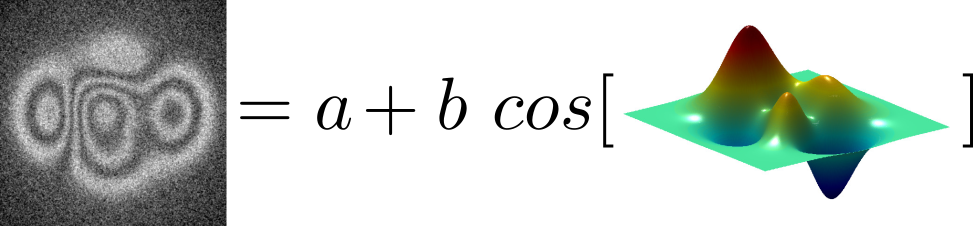
\includegraphics[scale=0.4]{Images/Interferogram.png}
  \end{center}
\end{frame}
%%%%%%%%%%%%%%%%%%%%%%%%%%%%
\begin{frame}{Algoritos de Cuadratura}
  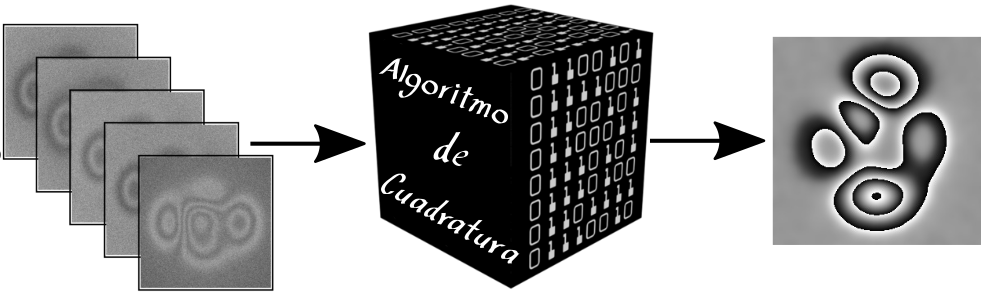
\includegraphics[scale=0.4]{Images/QuadratureFiltersScheme2.png}
\end{frame}
%%%%%%%%%%%%%%%%%%%%%%%%%%%%
\begin{frame}{Algoritos de Cuadratura}
\begin{center}

    \begin{eqnarray}
                      \mathcal{F}[I(x,y)] & = & I(\omega) \nonumber \\
                                                  & = & a\delta(\omega)+
                      \frac{b}{2}e^{-i \phi} \delta(\omega-\omega_0) +
                      \frac{b}{2} e^{i \phi} \delta(\omega+\omega_0)
    \end{eqnarray}
    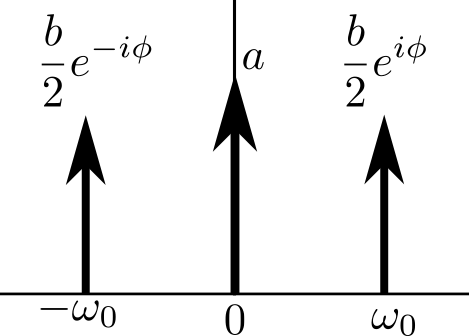
\includegraphics[scale=0.6]{Images/FourierDomine1.png}

\end{center}
\end{frame}
%%%%%%%%%%%%%%%%%%%%%%%%%%%%
\begin{frame}{Algoritos de Cuadratura}
\begin{center}

  \begin{equation}
            H(-\omega_0) =H(0) = 0, H(\omega_0) \neq 0
  \end{equation}
  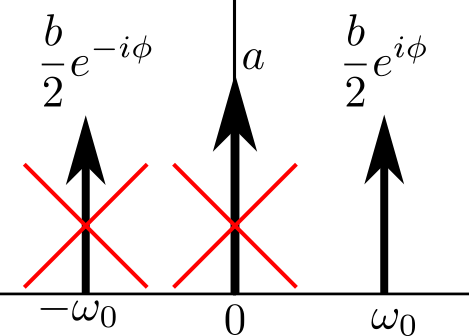
\includegraphics[scale=0.6]{Images/FourierDomine2.png} 

\end{center}
\end{frame}
%%%%%%%%%%%%%%%%%%%%%%%%%%%%
\begin{frame}{Algoritos de Cuadratura}
\begin{center}

    \begin{equation}
             I(\omega) H(\omega) = \frac{b}{2}exp[i \phi]
     \end{equation}
     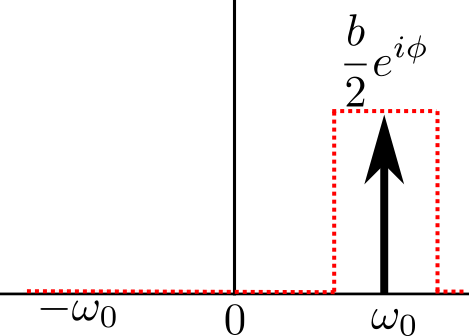
\includegraphics[scale=0.6]{Images/FourierDomine3.png}

  \end{center}
\end{frame}
%%%%%%%%%%%%%%%%%%%%%%%%%%%%
\begin{frame}{Algoritmos de Cuadratura}
\begin{center}

  \begin{equation}
    \hat \phi=atan\bigg[ \frac{ Im\{\frac{b}{2}exp[i \phi]\} }{
      Re\{\frac{b}{2}exp[i \phi]\} } \bigg]
  \end{equation}
  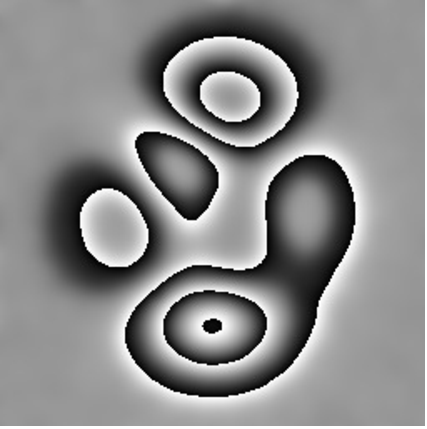
\includegraphics[scale=0.6]{Images/wPhase.pdf}

\end{center}
\end{frame}
%%%%%%%%%%%%%%%%%%%%%%%%%%%%
\begin{frame}{Filtros Regularizados}
\begin{center}

\begin{eqnarray}
  U[f(x,y)] &=&\iint_{(x,y) \in S} \Bigg\{ [f(x,y)-I(x,y)]^2 +  \nonumber \\
     & & \eta \bigg[  \frac{\partial ^2 f(x,y)}{\partial x^2} \bigg]^2 +
            \eta \bigg[  \frac{\partial ^2 f(x,y)}{\partial y^2} \bigg]^2 
     \Bigg\} dx dy
\end{eqnarray}
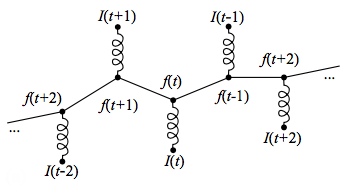
\includegraphics[scale=0.6]{Images/RegularizadosResorte.png}

\end{center}
\end{frame}
%%%%%%%%%%%%%%%%%%%%%%%%%%%%
\begin{frame}{Filtros Regularizados}
\begin{center}

\begin{eqnarray}
  U[f(x,y)] &=&\iint_{(x,y) \in S} \Bigg\{ [f(x,y)-I(x,y)]^2 + 
     \eta \bigg[  \frac{\partial ^2 f(x,y)}{\partial x^2} \bigg]^2 +
                \nonumber \\
      & &\eta \bigg[  \frac{\partial ^2 f(x,y)}{\partial y^2} \bigg]^2 +
     \eta \bigg[  \frac{\partial ^2 f(x,y)}{\partial x \partial y} \bigg]^2
     \Bigg\} dx dy
\end{eqnarray}
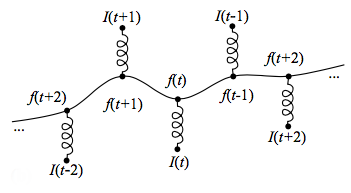
\includegraphics[scale=0.6]{Images/RegularizadosPlaca.png}

\end{center}
\end{frame}
%%%%%%%%%%%%%%%%%%%%%%%%%%%%
\begin{frame}{Filtros Regularizados}
\begin{center}

\begin{equation}
  U[f(x,y)]= \sum_{(x,y) \in S} \Big\{  [ f(x,y)-I(x,y) ]^2 + \eta R[f(x,y)] \Big\} 
\end{equation}
Resorte:
\begin{equation}
  R_r [f(x,y)] = [f(x,y)-f(x-1,y)]^2 + [f(x,y)-f(x,y-1)]^2 
\end{equation}

Placa:
\begin{eqnarray}
  R_p [f(x,y)] & = & [f(x+1,y)-2f(x,y)-f(x-1,y)]^2 \nonumber \\
  & & + [f(x,y+1)-2f(x,y)-f(x,y-1)]^2 \nonumber \\
  & & + [ f(x+1,y+1)-f(x-1,y-1) \nonumber \\ 
  & & + f(x-1,y+1)-f(x+1,y-1) ]^2
\end{eqnarray}

\end{center}
\end{frame}
%%%%%%%%%%%%%%%%%%%%%%%%%%%%
\begin{frame}{Filtros Regularizados}
\begin{center}

Resorte:\\
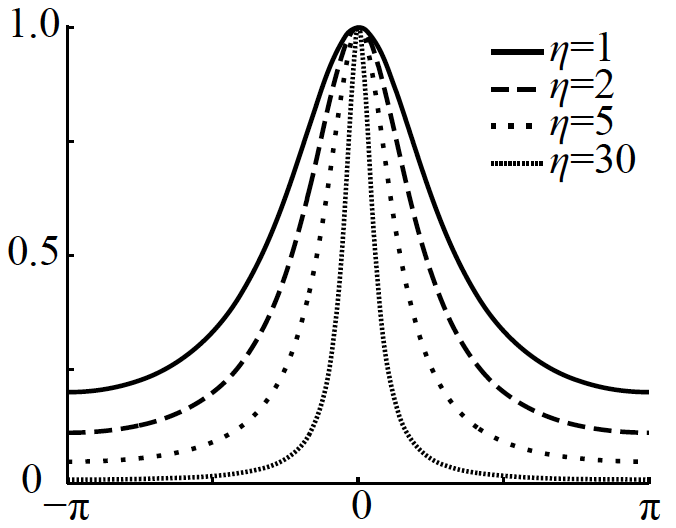
\includegraphics[scale=0.6]{Images/FrecuenciaResorte.png}

\end{center}
\end{frame}
%%%%%%%%%%%%%%%%%%%%%%%%%%%%
\begin{frame}{Filtros Regularizados}
\begin{center}

Placa:\\
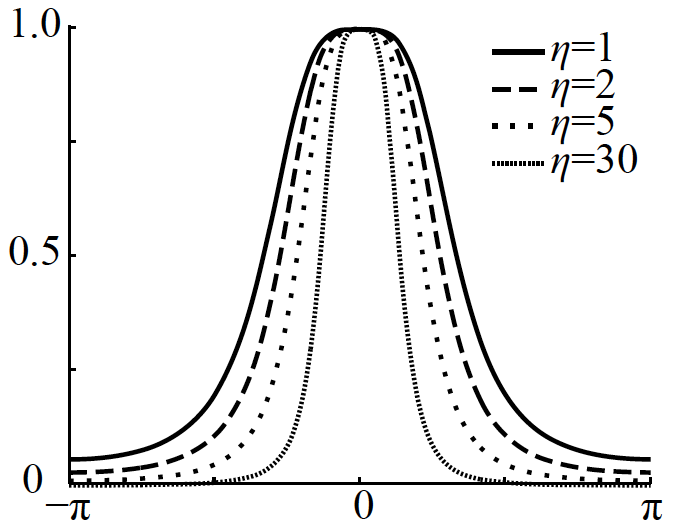
\includegraphics[scale=0.6]{Images/FrecuenciaPlaca.png}

\end{center}
\end{frame}
%%%%%%%%%%%%%%%%%%%%%%%%%%%%
\begin{frame}{Filtros Regularizados}
\begin{center}


\end{center}
\end{frame}
%%%%%%%%%%%%%%%%%%%%%%%%%%%%

\end{document}